\documentclass[11pt]{amsbook}

\makeatletter
\def\@thm#1#2#3{%
  \ifhmode\unskip\unskip\par\fi
  \normalfont
  \trivlist
  \let\thmheadnl\relax
  \let\thm@swap\@gobble
  \let\thm@indent\indent % indent
  \thm@headfont{\bfseries}% heading font boldface // changed
  \thm@notefont{\fontseries\mddefault\upshape}%
  \thm@headpunct{.}% add period after heading
  \thm@headsep 5\p@ plus\p@ minus\p@\relax
  \thm@space@setup
  #1% style overrides
  \@topsep \thm@preskip               % used by thm head
  \@topsepadd \thm@postskip           % used by \@endparenv
  \def\@tempa{#2}\ifx\@empty\@tempa
    \def\@tempa{\@oparg{\@begintheorem{#3}{}}[]}%
  \else
    \refstepcounter{#2}%
    \def\@tempa{\@oparg{\@begintheorem{#3}{\csname the#2\endcsname}}[]}%
  \fi
  \@tempa
}
\makeatother

\renewcommand{\chaptername}{Lecture}


\usepackage[T1]{fontenc}
\usepackage[latin1]{inputenc}
\usepackage{times}
\usepackage{microtype}
\usepackage{amssymb}
\usepackage{a4wide}
\usepackage{graphicx}
%\usepackage{paralist}
\usepackage{bbm}
\usepackage{color}
\usepackage[pagebackref]{hyperref} 
\hypersetup{pdftitle={\title}, pdfauthor={\author}}
\usepackage{verbatim}
\usepackage{url}
\usepackage[pagebackref]{hyperref}
\hypersetup{pdftitle={\title}, pdfauthor={\author}}

\usepackage{amsmath}
%\usepackage{mathtools}
\usepackage{tikz}
\usetikzlibrary{matrix,arrows,decorations.pathmorphing}

\newcommand{\ba}{{\boldsymbol{a}}}
\newcommand{\balpha}{{\boldsymbol{\alpha}}}
\newcommand{\bb}{{\boldsymbol{b}}}
%\newcommand{\bc}{{\boldsymbol{c}}}
\newcommand{\be}{{\boldsymbol{e}}}
\newcommand{\bff}{{\boldsymbol{f}}}
\newcommand{\bnu}{{\boldsymbol{\nu}}}
\newcommand{\bm}{{\boldsymbol{m}}}
\newcommand{\bo}{{\boldsymbol{0}}}
\newcommand{\bp}{{\boldsymbol{p}}}
\newcommand{\bq}{{\boldsymbol{q}}}
\newcommand{\br}{{\boldsymbol{r}}}
\newcommand{\bsigma}{{\boldsymbol{\sigma}}}
\newcommand{\bt}{{\boldsymbol{t}}}
\newcommand{\bv}{{\boldsymbol{v}}}
\newcommand{\bw}{{\boldsymbol{w}}}
\newcommand{\bx}{{\boldsymbol{x}}}
\newcommand{\by}{{\boldsymbol{y}}}
\newcommand{\bz}{{\boldsymbol{z}}}
\newcommand{\bone}{{\boldsymbol{1}}}

\newcommand{\RR}{\mathbb{R}}
\newcommand{\Rgeo}{{\mathbb{R}_{\ge0}}}
\newcommand{\Zgeo}{{\mathbb{Z}_{\ge0}}}
\newcommand{\NN}{\mathbb{N}}
\newcommand{\ZZ}{\mathbb{Z}}
\newcommand{\QQ}{\mathbb{Q}}
\newcommand{\CC}{\mathbb{C}}

\newcommand{\cA}{{\mathcal{A}}}
\newcommand{\cC}{{\mathcal{C}}}
\newcommand{\cD}{{\mathcal{D}}}
\newcommand{\cH}{{\mathcal{H}}}
\newcommand{\cL}{{\mathcal{L}}}
\newcommand{\cO}{{\mathcal{O}}}
\newcommand{\cP}{{\mathcal{P}}}

\newcommand{\cU}{\mathcal{U}}
\newcommand{\tU}{\tilde{\mathcal{U}}}
\newcommand{\tV}{\tilde{\mathcal{V}}}

\newcommand{\scp}[2]{\langle #1,#2\rangle}
\newcommand{\fl}[1]{\left\lfloor #1\right\rfloor}
\newcommand{\ce}[1]{\left\lceil #1\right\rceil}
\newcommand{\rcone}[1]{{{}_\Rgeo\!\left\langle #1\right\rangle}}
\newcommand{\zcone}[1]{{{}_\Zgeo\!\left\langle #1\right\rangle}}

\newcommand{\bn}{{\color{blue}\texttt{\bfseries n}}}
\newcommand{\bc}{{\color{blue}$\boldsymbol{\circ}$}}
\newcommand{\rn}{{\color{red}\texttt{\bfseries n}}}
\newcommand{\rs}{{\color{red}\texttt{\bfseries *}}}
\newcommand{\rt}{{\color{red}$\boldsymbol{\times}$}}
\newcommand{\bB}{{\color{blue}\texttt{\bfseries B}}}
\newcommand{\rR}{{\color{red}\texttt{\bfseries R}}}

\newcommand{\crb}[1]{{\color{red}\texttt{\bfseries{#1}}}}
\newcommand{\cbb}[1]{{\color{blue}\texttt{\bfseries{#1}}}}

\DeclareMathOperator{\interior}{int}
\DeclareMathOperator{\relint}{relint}
\DeclareMathOperator{\conv}{conv}
\DeclareMathOperator{\cone}{cone}
\DeclareMathOperator{\aff}{aff}
\DeclareMathOperator{\vol}{vol}
\DeclareMathOperator{\dist}{dist}
\DeclareMathOperator{\vertices}{vert}
\DeclareMathOperator{\rang}{rang}
\DeclareMathOperator{\sign}{sign}
\DeclareMathOperator{\pyr}{pyr}
\DeclareMathOperator{\bipyr}{bipyr}
\DeclareMathOperator{\Sl}{Sl}
\DeclareMathOperator{\im}{Im}
\DeclareMathOperator{\colspan}{colspan}
\DeclareMathOperator{\rank}{rank}

%%%%%%%%%%%%%%%%%%%%%%%%%%%%%%%%%%%%%%%%Ferran%%%%%%%%%%%%%%%%%%%%%%%%%%%%%%%%%%%%%%%%%%%%%%%%%%%%%%%%%%%%%%%%%%%%%%%%%%%%%%%
\newcommand{\Proj}{\mathbb{P}}
\DeclareMathOperator{\id}{id}
\DeclareMathOperator{\Vor}{Vor}
\newcommand{\HH}{\mathbb{H}}

\DeclareMathOperator{\sgn}{sgn} %signum
\DeclareMathOperator{\ggT}{ggT}

\newcommand{\ojo}[1]{\textsf{\bfseries\boldmath #1}}
\newcommand{\scribe}[1]{\begin{center}\emph{Scribe: #1}\end{center}\bigskip}

\graphicspath{{graphics/}}

\numberwithin{equation}{chapter}

\newtheorem{theorem}{\textbf{Theorem}}[chapter]
\newtheorem{lemma}[theorem]{Lemma}
\newtheorem{proposition}[theorem]{Proposition}
\newtheorem{corollary}[theorem]{Corollary}
\newtheorem{conj}[theorem]{Conjecture}
\newtheorem{exercise}[theorem]{Exercise}
\newtheorem{example}[theorem]{Example}
\newtheorem{claim}[theorem]{Claim}

\theoremstyle{definition}
\newtheorem{definition}[theorem]{Definition}
\newtheorem{defn}[theorem]{Definition}
\newtheorem{remark}[theorem]{Remark}
\newtheorem{observation}[theorem]{Observation}
\newtheorem{obs}[theorem]{Observation}

%\includeonly{lecture3}

\begin{document}

\thispagestyle{empty}

\newcommand{\thisyear}{2013}

\
\vfill
\begin{center}
        \Huge \sffamily\bfseries 
        Discrete and Algorithmic Geometry \thisyear
        \medskip
        (Part 2)

\vspace{2cm}
\LARGE
Julian Pfeifle

\vspace{3cm}

\normalfont\LARGE\sffamily
Version of \today

\vspace{5cm}\
\end{center}

This is the preliminary version of the lecture notes for the second
part of \emph{Discrete and Algorithmic Geometry} (Universitat
Polit�cnica de Catalunya), held in the fall semester of \thisyear\ by Ferran
Hurtado and Julian Pfeifle.

\medskip
These notes are fruit of the collaborative effort of all participating
students, who have taken turns in assembling this text. The name of
each scribe figures in each corresponding section.

\medskip
%The main literature for this course consists of
%\cite{Conway-Sloane-3rd}, \cite{Conway-Strauss08}
%and~\cite{Senechal95}. 

\medskip Suggestions for improvements will always be gladly received
by \texttt{julian.pfeifle@upc.edu}.

\vfill\


% Local Variables: 
% mode: latex
% TeX-master: "dag-upc"
% End: 

\tableofcontents

\chapter{Convex Polytopes}

\scribe{Cecilia Girón}
 
A convexpolytope can be defined in two different ways:
\begin{enumerate}
\item[-] \textit{$V$-polytope} (discrete geometry): is the convex hull of the finite non-empty point set in $\mathbf{R}^d$.
\item[-]\textit{$H$-polytope} (linear/integer optimization): An $H$-polyhedron is an intersection of a finite number of linear half spaces in some $\mathbf{R}^d$, if non-empty. And a $H$-polytope is a bounded $H$-polyhedron. 
\end{enumerate}
\bigskip
\subsection{Faces}
One of the properties studied about polytopes is their faces. A \textbf{face} $F$ of a polytope $P$ is a set of the form:
\[F ) \{x\in \mathbb{R}^d: <a,x> = n\}\cap P\]
where $a\in (\mathbb{R}^d)^*$ (dual space), $b\in\mathbb{R}$ and $P\subseteq\{x\in\mathbb{R}^d: <a,x> \leq b \}\longleftrightarrow$ The inequality $<a,x> \leq b$ is valid for $P$. Notice that $P$ is actually a face of itself. 

We can also study the of a face $dim F$. Let $P$ be a $d$ dimensional polytope, then if a face $F$ of $P$ has dimension:
\begin{itemize}
\item[i)] $d -1$ is called \textbf{facets}.
\item[ii)] $d -2$is called \textbf{ridges}.
\item[iii)] $1$ is called \textbf{edge}.
\item[iv)] $0$ is called \textbf{vertex}.
\item[v)] $ -1$ then $F=\emptyset$.
\end{itemize}

The parial ordering set of all faces  $\mathcal{F}(P)$ of a convex polytope $P$ form an Eulerian lattice called \textbf{face lattice}. Face lattice can be used, for instance, to count the number of faces of same dimension:
\[f_i = \# \{ \mbox{ faces } F \mbox{ of } P \mbox{ with } dimF=i\} \label{eq1}\]

\bigskip

\textsc{Example}. Let $P$ be a cube in two dimensions, so a square. Notice that $dim P = 2$, for every edge $ij\in P$ $dim(ij) = 1$ and for every vertex $i$ $dim i= 0$, for $i,j= 1, 2 , 3,4$ and $i\neq j$. With this information we can construct the face lattice and study some properties of $P$.

\begin{figure}[h!]
\begin{minipage}[t]{0.4\textwidth}
   \vspace{30pt}
   \hspace{20pt}

\begin{picture}(100,100)
\put(115,0){4}
\put(0,1){3}
\put(0,100){1}
\put(115,100){2}
\put(8,105){\textbullet}
\put(108,105){\textbullet}
\put(8,8){\textbullet}
\put(108,8){\textbullet}
\multiput(10,10)(100,0){2}{\line(0,100){100}}
\multiput(10,10)(0,100){2}{\line(100,0){100}}
\end{picture}

\end{minipage}
  \hfill
\begin{minipage}[t]{0.6\textwidth}
      \vspace{0pt}
      \hspace{-100pt}
\[
\xymatrix{
& & P\ar[dr]\ar[drr]\ar[dl]\ar[dll] & & & f_2 = 1 \\
13\ar[d]\ar[drrrr]  & 12\ar[d]\ar[dl]&  & 24\ar[d]\ar[dll] & 34\ar[d]\ar[dl] & f_ 1 = 4\\
1\ar[drr]  & 2\ar[dr]&  & 3\ar[dl] & 4\ar[dll] & f_0=4\\
 & & \emptyset & & & F_{-1}=1
 }
\]
\end{minipage}
\end{figure} 


\begin{flushright}
$\clubsuit$
\end{flushright}

\bigskip
\textsc{Example}.Let's study now the dimension of the faces of a hypercube of dimension d $\square ^d = \{ x\in\mathbb{R}^d: -1\leq x_i\leq 1, i=1,\cdots, d\}$: $f_{-1}(\square ^d) = 1, f_{0}(\square ^d) = 2^d,f_{d-1}(\square ^d) = 2d $ and $f_{d}(\square ^d) = 1$. Notice that the radius $r$ from the center of the cube to one of its vertices is $r=\sqrt{d}-1$, thus the exterior circus of the polytope has radio $r$ and the interior radio 1. 
\bigskip



\begin{tabular}{| c | c | c | c | c | c | c | c | c |}
  \hline                        
  d & 2 & 3 & 4 & 5 & $\cdots$ & 100 & $\cdots$ & $10^{100}$ \\
  \hline 
 $r=\sqrt{d}-1$ & $\sqrt{2}-1$ & $\sqrt{3}-1$ & $1$ & $\sqrt{5}-1$ & $\cdots$ & 9  & $\cdots$ & $10^{50}-1$ \\
  \hline  
  $f_0$ & $4$ & $8$ & $16$  & $32$ &  $\cdots$ & $2^{100}$ &  $\cdots$ & $2^{10^{100}}$ \\
  \hline
  $f_{1}$ & $4$ & $6$ & $8$  & $10$ &  $\cdots$ & $200$ &  $\cdots$ & $2\cdot 10^{100}$ \\
  \hline  
\end{tabular}

\begin{flushright}
$\clubsuit$
\end{flushright}

\bigskip

An other property that can be studied about the faces of convex polytopes is whether they are a simplex or not. Let $P$ be a polytope such that $dim P = d$ and $\mathcal{F}(p) = k+1$. It is said to be \textbf{simplicial} if it is $k$-simplex, i.e. if each of its faces is a simplex; and it is called \textbf{simple} if each of its vertices is contained in exactly $d$ faces where $dim P =d$.

\bigskip
\textbf{Exercises done during the lecture 8/11/2013. Each one includes one}


\subsection{Asymptotic f-vectors of families of polytopes}

In this section we are going to study the \textit{unimodal conjecture} which says that there exists an $l = P(L)\in\mathbb{N}$ such that $f_0\leq f_1 \leq \cdots\leq f_l \leq f_{l+1}\leq \cdots \leq f_{d-1}\leq f_d$. We woould like to know if it is true. 

First, we define the \textbf{$f$-vector} as the vector of the form $(f_0,f_{1},\cdots,f_{d-1})$ where $f_i$ is as defined before in (\ref{eq1}). We will say that it is a \textbf{flag $f$-vector} $(f_s)_s = [d]$ such that $f_s$ count the number of flags $F_{i_1} \subset F_{i_2} \subset \cdots \subset F_{i_k}$ where $s = \{i_1,i_2,\cdots, i_k \}$ and $dim F_{i_k} = i_k$ \footnote{You can also read about $cd$-index}.

\bigskip
The unimodal conjecture described before is known to be false for simplical polytopes of dimension $d\geq 19$ and for non-simplicial polytopes of dimension $d \geq 8$. The following conjecture is not known to be false. 

\textbf{Restricted unimodal conjeture (Anders Bjorner)}: 
\begin{eqnarray*}
 f_0\leq f_1\leq \cdots \leq f_{\lfloor \frac{d-1}{4}}\rfloor\\
 f_{\lfloor \frac{3(d-1)}{4}\rfloor}\geq \cdots \geq f_{d-1}
\end{eqnarray*} 

Intuitively we are sure that there is no way this conjecture could be false, but there is not proof of this. We don't even know if $f_k\geq \frac{1}{10000}\min\{f_0,f_{d-1}\}$ is true.

\bigskip

\textbf{Exercises done during the lecture 11/11/2013. Each one includes one}


\subsubsection{Operations on polytopes}
\begin{itemize}
\item \textbf{Cartesian (direct) product} $P\times Q$.
\item \textbf{Direct sum} $P^d \oplus q^e \subset \mathbb{R}^{d+e}$.
\item $P*Q\subset \mathbb{R}^{d+e+1}$. It is like $\oplus$ but the subspaces are skew (i.e. affine and they have no point on common). For example $\square^1 *\square^1 = Pyr(P)$.
\end{itemize}

\bigskip
\noindent\textsc{Example}: Given $f_k(P)$, calculate the $k$-th entry of $Pyr(P)$:
\begin{eqnarray*}
f(P)&=&(f_0,f_1,\cdots, f_{d-1}\\
f_k(Pyr(P)) &=& (f_0 +1, f_1 + f_0, f_2+f_1, \cdots, f_{d-2}+ f_{d-3}, f_{d-1}+ f_{d-2}, 1+ f_{d-1})
\end{eqnarray*}
\begin{flushright}
$\clubsuit$
\end{flushright}

\bigskip
\begin{itemize}
\item  \textbf{Connected sum} $P^d\#Q^d$ where $P$ has as simplicial face $f$ and $Q$ has a simplicial face $G$. 
\end{itemize}

This last operation is used to join the asymptotic function $f(\square^d)$ and its dual $f(\diamondsuit ^d)$. To make it work, since $\square^d$ has no triangulations in its faces, it is enough to cut away one vertex and, this way, get a simplex. Merging both functions using the connected sum gives place to a new function which is a non-unimodal function.

% Local Variables: 
% mode: latex
% TeX-master: "dag-upc"
% End: 

\chapter{Volumes of balls and cubes; Lattice Polytopes}

\scribe{Victor Bravo}

\section{Comparing the volumes of balls and cubes}

Given an $n$-dimensional ball of radius $r$, we have that
$\text{vol}(B^{n}_{r}) = \dfrac{\pi^{\frac{n}{2}}}{\Gamma(\frac{n}{2}
  + 1)}r^{n}$, where $\Gamma$ is the Gamma Function, which is defined
in the following way:

\begin{enumerate}

\item $\Gamma(m + 1) = m !$, for $m \in \mathbb{N}_{0}$.

\item $\Gamma(m + \frac{1}{2}) = \dfrac{(2m)!}{m! 4^{m}}\sqrt{\pi}$.
\end{enumerate}

\begin{example} $\text{vol}(B^{1}_{r}) = \dfrac{\sqrt{\pi}}{\Gamma(1 + \frac{1}{2})}r = \dfrac{1!\sqrt{\pi}4^{1}}{2!\sqrt{\pi}}r = 2r$.
\end{example}
\begin{example} $\text{vol}(B^{2}_{r}) = \dfrac{\pi}{1!}r^{2} = \pi r^{2}$.
\end{example}

Now, we want to know the asymptotic behaviour, i.e., having a cube
with a ball inside, we want to know how evolves the volume of the cube
compared with the volume of the ball. Using the unit cube, in
dimension $1$, we have the same volume for the cube and the ball
because they are the same thing. In dimension $2$ (see figure 1), we
have a square with every edge of length $1$ and then, the ball has
radius $1/2$. In dimension $3$ (see figure 2), we have a cube with
every edge of length $1$ and then, the ball also has radius $1/2$,
etc.

\begin{figure}
\centering
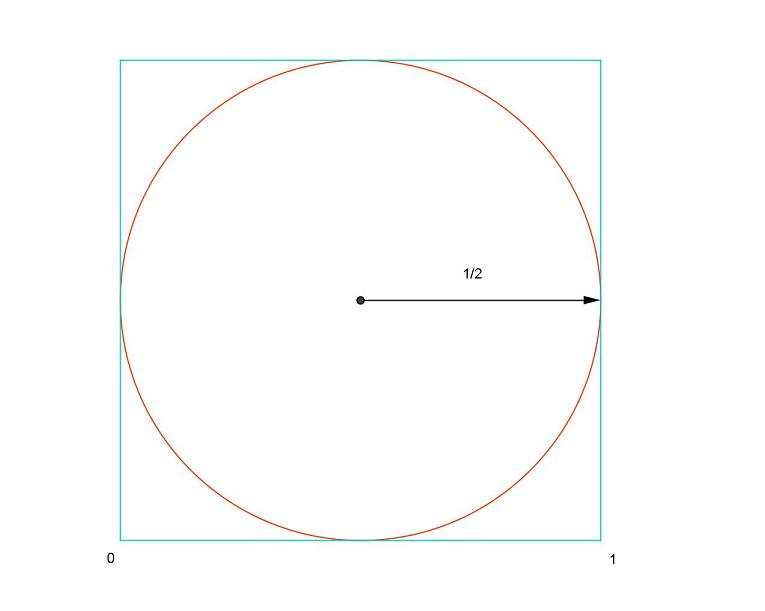
\includegraphics[width=0.5\textwidth]{figure1.jpg}
\caption{Example in dimension $2$.}
\end{figure}

\begin{figure}
\centering
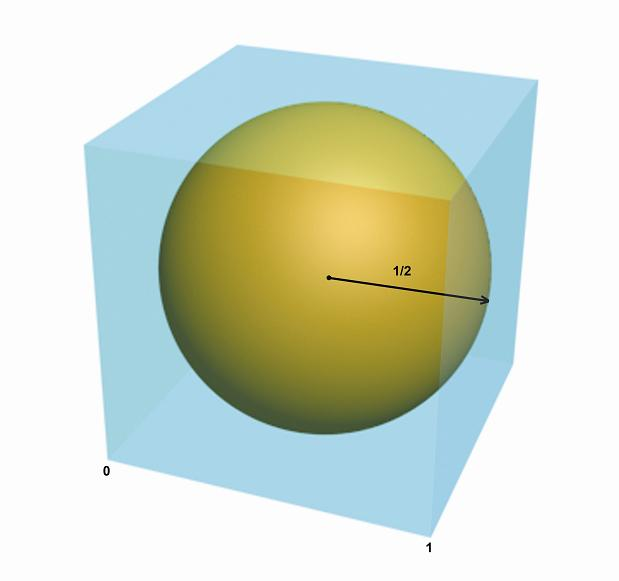
\includegraphics[width=0.5\textwidth]{figure2.jpg}
\caption{Example in dimension $3$.}
\end{figure}

Then, the general case is,
$\dfrac{\text{vol}(B^{n}_{1/2})}{\text{vol}(_{0}^{}\square_{1}^{n})} =
\text{vol}(B_{1/2}^{n}) =$ fraction of unit cube taken up by largest
ball contained inside.

Now, using Stirling's approximation, $\Gamma(x + 1) \approx \sqrt{2
  \pi x}\left(\dfrac{x}{e}\right)^{x}$, $x \in \mathbb{R}_{\geq 0}$,
we have that asymptotically,

$\text{vol}(B_{1/2}^{n})
\stackrel{n \rightarrow \infty}{\longrightarrow}
\dfrac{\pi^{\frac{n}{2}}(\frac{1}{2})^{n}}{\sqrt{2 \pi\frac{n}{2}}(\frac{n/2}{e})^{\frac{n}{2}}} =
\dfrac{\pi ^\frac{n}{2} 2^\frac{n}{2} e^\frac{n}{2}}{\sqrt{\pi n} n^\frac{n}{2} 2^{n}} =
\dfrac{1}{\sqrt{\pi n}}\left( \dfrac{\pi e}{2n} \right)^{\frac{n}{2}} 
\stackrel{n \rightarrow \infty}{\longrightarrow}
0$.

\begin{example} $\dfrac{\text{vol}(B_{1/2}^{100})}{\text{vol}(\square^{100})} \approx 10^{-67}$.
\end{example}

Then, we have bad news for numerical integration (for example in the
case of Monte Carlo integration) when it is used in physics or in
financial mathematics because, by the example above, we will be not
able to count from $1$ to $10^{-67}$. This is too long. So, this works
worst as the dimension increases. In conclusion, we will not use Monte
Carlo Integration to calculate volumes in high dimensions because the
volumes of the balls will be so tiny.

\begin{remark} An example of Monte Carlo Integration in physics
  consists in throw random points into our space and count how many
  points fall inside and how many points fall outside. Then, do the
  fraction which divides the number of points inside and the number of
  points thrown and this fraction approximates the volume (it is used
  at CERN). In the other hand, Monte Carlo Integration is used in
  financial mathematics, for example if we have a portfolio with many
  variables and we have to integrate, one way to integrate by all this
  variables is using Monte Carlo Integration.
\end{remark}


\section{Lattices and lattice polytopes}

Now, we will talk about lattice packings of spheres. A lattice has two
different meanings in mathematics: a partially ordered set or a
group. We are gonna talk about the group.

The most important lattice is $\mathbb{Z}^{d}$, and it's called the
integer lattice. This is an abelian group with the sum: $x, y \in
\mathbb{Z}^{d} \Rightarrow - x \in \mathbb{Z}^{d}, x + y \in
\mathbb{Z}^{d}$, and the sum is commutative.

Now, if we have $v_{1}, \ldots, v_{n} \in \mathbb{Z}^{d}$, and we have
a look to $P = \text{conv}\lbrace v_{1}, \ldots, v_{n} \rbrace
\subseteq \mathbb{R}^{d}$, we define a lattice polytope as the convex
hull of a finite set of points with integer coordinates.

\begin{figure}
\centering
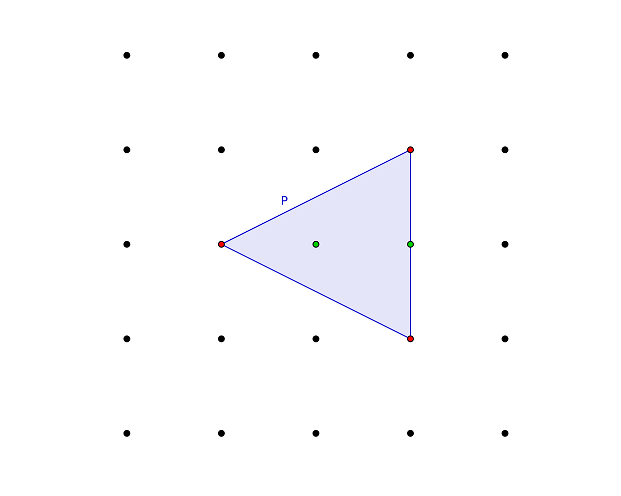
\includegraphics[width=0.5\textwidth]{figure3.png}
\caption{A lattice triangle.}
\end{figure}

Now, we can do the next question: When two lattice triangles "the
same"? The first observation is that we have to answer is: When two
polytopes are "the same"? In Figure 4, we can say that the two lattice
triangles are "the same" because they share all properties respect to
the lattice.

\begin{figure}
\centering
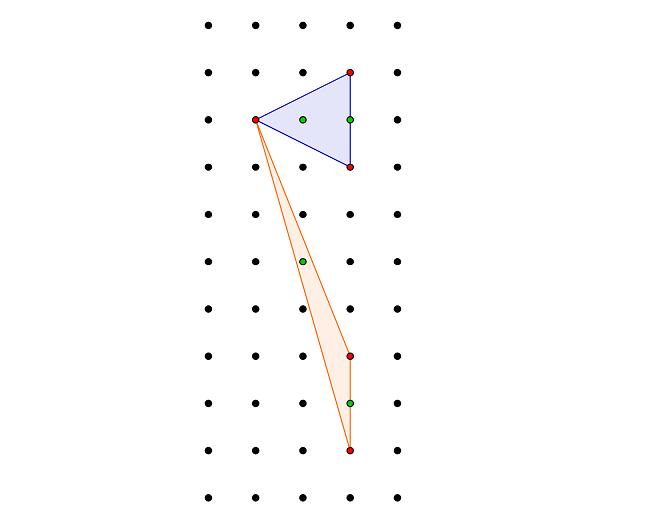
\includegraphics[width=0.5\textwidth]{figure4.png}
\caption{Two lattice triangles.}
\end{figure}

Now, forgetting lattices, the answer to the question for polytopes in
general is: Klein's Erlangen Program. In this program, Klein
identifies the geometry with the groups of automorphisms, i.e., what
Klein makes is to say what the geometry is, by seeing which group of
automorphisms leaves certain object invariant.

Some groups that we must have in mind are $O(n, \mathbb{R}) = \lbrace
A \in \mathbb{R}^{n \times n} : A^{-1} = A^{T} \rbrace$ and $SO(n,
\mathbb{R}) = O(n, \mathbb{R}) \cap \lbrace A \in \mathbb{R}^{n \times
  n} : \det A = 1 \rbrace$. In the other hand, we can also have in
mind the set of translations in $\mathbb{R}^{n \times n}$, $T(n,
\mathbb{R}^{n \times n})$, which satisfies $SO(n, \mathbb{R}^{n \times
  n}) \rtimes T(n, \mathbb{R})$, where $\rtimes$ is the semi-direct
product, which means: two subsets, $P, Q \subseteq \mathbb{R}^{n}$,
are ''the same'' if $\exists A \in O(n)$ and $\exists t \in
\mathbb{R}^{n} : Q = A \cdot P + t$, i.e., I can obtain $Q$ from $P$
through a rotation $A$ and a translation $t$ (i.e., $P$ and $Q$ are
congruent), and this is what we know as Euclidean Geometry.

Now, remembering lattices, we have to change the euclidean geometry by
lattice geometry, i.e., we want bijective homomorphisms that preserves
the lattices. So, we want to determine $\text{Aut}(\mathbb{Z}^{d}) =
\lbrace \text{affine transformations that leave } \mathbb{Z}^{d}
\text{ invariant} \rbrace$, and this is to find conditions on $A \in
\mathbb{R}^{n \times n}$ and $t \in \mathbb{R}^{n}$ such that $Ax + t
\in \mathbb{Z}^{d}$, $\forall x \in \mathbb{Z}^{d}$.
These conditions are:

\begin{itemize}
\item $x = 0$, want $A \cdot 0 + t \in \mathbb{Z}^{d}
  \Longleftrightarrow t \in \mathbb{Z}^{d}$.

\item $x = e_{i}$, with $e_{i}$ a generating vector of our lattice,
  want $A \cdot e_{i} \in \mathbb{Z}^{d} \Longleftrightarrow$ every
  column of $A \in \mathbb{Z}^{d} \Longleftrightarrow A \in
  \mathbb{Z}^{d \times d}$.
\end{itemize}

Now, for $A$ to be an automorphism, it must be invertible, and
$A^{-1}$ must belong to $\mathbb{Z}^{d \times d}$.

\begin{example} Suppose that $d = 2$. We have
  $\left( \begin{smallmatrix} a & b \\ c & d \end{smallmatrix} \right)
  \in \mathbb{Z}^{2 \times 2}$. Then, $A^{-1} = \frac{1}{ad - bc}
  \left( \begin{smallmatrix} d & -b \\ -c & a \end{smallmatrix} \right) =
  \frac{1}{\det A}\left[ (c_{ij}) \right]$, where $(c_{ij})$
  represents the cofactors of $A$. And $A^{-1} \in \mathbb{Z}^{2
    \times 2}$ because $ad - bc$ never divides the entries of
  $\left( \begin{smallmatrix} d & - b \\ - c & a \end{smallmatrix}
  \right)$. (This has to be proved.)
\end{example}

Then, $\text{Aut}(\mathbb{Z}^{d}) = \left\lbrace A \in \mathbb{Z}^{d
    \times d} : \det A = \pm 1 \right\rbrace \rtimes \mathbb{Z}$.

Observe that the set of orientation-preserving linear (not affine)
automorphisms of $\mathbb{Z}^{d}$ is $\Sl_d(\ZZ) = \big\{ A \in
\mathbb{Z}^{d \times d} : \det A = 1 \}$, the special linear group
with integer coefficients. On the other hand, $\left\lbrace A \in
  \mathbb{Z}^{d \times d} : \det A = -1 \right\rbrace$ is not a group.

  Then, what lattice geometry means is that geometry with group
  automorphisms: $Sl_{d}(\mathbb{Z}) \rtimes \mathbb{Z}^{d}$, and this
  is mapping $x \longmapsto Ax + t$, with $t \in \mathbb{Z}^{d}$, $A
  \in \mathbb{Z}^{d \times d}$, and $\det A = \pm 1$. Then, any two
  lattice polytopes in correspondence by any of this automorphisms
  will be the same polytope.

  Now, observe that in Figure 4, using that the image of the vectors
  are the same than the columns of the matrix $A$, we have that $A =
  \left[ \begin{smallmatrix} 1 & 0 \\ -2 & 1 \end{smallmatrix}
  \right]$, with $A \cdot e_{1} = \left( \begin{smallmatrix} 1 \\ -
      2 \end{smallmatrix}
  \right)$ and $A \cdot e_{2} = \left( \begin{smallmatrix} 0 \\
      1 \end{smallmatrix} \right)$.  Also, observe that the following
  transforms (called \emph{shears}) are typical lattice transforms in
  $\mathbb{Z}^{2}$: $\left[ \begin{smallmatrix} 1 & 0 \\ * &
      1 \end{smallmatrix} \right]$ and $\left[ \begin{smallmatrix} 1 &
      * \\ 0 & 1 \end{smallmatrix} \right]$. This can be used in
  exercise 3 of list 1.

After seen this, we are going to see some definitions:

Let $P \subseteq \mathbb{R}^{d}$ be a polytope ($\sim$ convex hull of
finitely many points). A linear inequality of the form $ax \leq b$
with $a \in (\mathbb{R}^{d})^{*}$, $x \in \mathbb{R}^{d}$, $b \in
\mathbb{R}$ is valid for $P$ if all points of $P$ satisfy it. (observe
that $(\mathbb{R}^{d})^{*}$ represents the dual space of
$\mathbb{R}^{d}$).

A face of $P$ is $P \cap \lbrace x \in \mathbb{R}^{d} : ax = b
\rbrace$, where $ax \leqslant b$ is a valid linear inequality for
$P$. In particular, $\emptyset$ is always a face of $P$ (example: $0x
\leqslant 1$), and $P$ is always a face of $P$ (example: $0x \leqslant
0$). This, bring us to a second meaning of lattice:

The face lattice of $P$ is the poset (partially ordered set) of faces
of $P$ with the inclusion.

\begin{example} If we have the polytope of figure 5, this polytope
  will have the face lattice of figure 6 (where O represents the
  $\emptyset$).
\end{example}

\begin{figure}
\centering
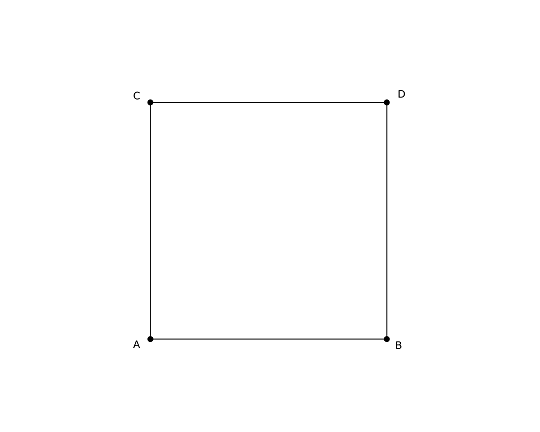
\includegraphics[width=0.5\textwidth]{figure5.png}
\caption{Square ABCD.}
\end{figure}

\begin{figure}
\centering
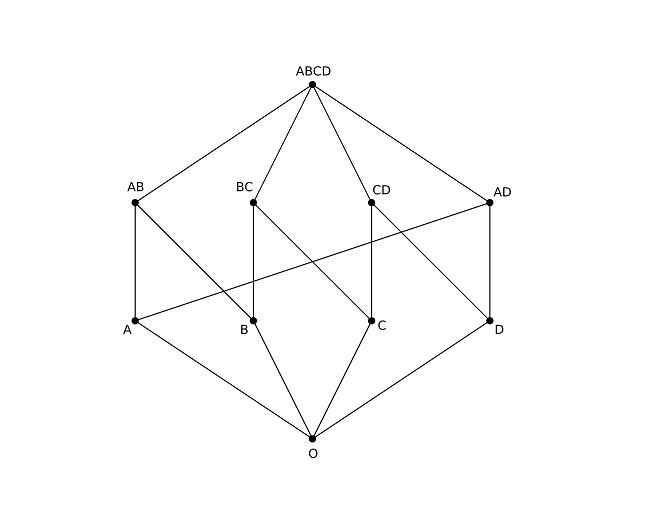
\includegraphics[width=0.5\textwidth]{figure6.png}
\caption{Its face lattice.}
\end{figure}


If anybody wants to read about this, then read ''Lectures on
Polytopes'' by Ziegler.

This can be applied to cubes, for example, as follows:

\begin{center}
  $(1 0 0 0 1 1)\left( \begin{array}{c} x_{1} \\ x_{2} \\ x_{3} \\
      x_{4} \\ x_{5} \\ x_{6} \end{array} \right) \leqslant k$,
\end{center}

where $k$ represents the non-zero entries (in this case $k = 3$), and
using this, we can calculate the barycenters.


% Local Variables: 
% mode: latex
% TeX-master: "dag-2011"
% End: 
 
\chapter{Pick's Theorem; Lattice packings of spheres}

\scribe{Miquel Ra\"{i}ch}

\section{Pick's Theorem}
\begin{theorem}[Pick]
Let $P$ be a lattice polygon in the plane ($P$ is closed, convex, simple and its vertices lie in $\ZZ^{2}$).
The area of $P$ is $$A(P)=\vol_{2}P=I+\frac{1}{2}B-1$$where:\\
$\mbox{    }\mbox{    } I=$ number of interior lattice points of $P$ $=\#\left\{(\mbox{int }P)\cap\ZZ^{2}\right\}$,\\
$\mbox{    }\mbox{    } B=$ number of boundary lattice points of $P$ $=\#\left\{\partial{}P\cap\ZZ^{2}\right\}$
\end{theorem}
\begin{proof}\mbox{[part]}\\
\begin{enumerate}
\item Show that Pick's formula is additive: if $P=P_1\cup{}P_2$, then $$I+\frac{1}{2}B-1=\left(I_1+\frac{1}{2}b_1-1\right)+\left(I_2+\frac{1}{2}B_2-1\right)$$
\begin{align*}A(P)=&A(P_1)+A(P_2)\\
I=I(P)=&I_1+I_2+L-2\\
B=B(P)=&B_1+B_2-2L+2\end{align*}
{\center (Principle of Inclusion-Exlusion $\rightarrow$ M\"obius function)\quad\quad\\[0.3cm]

\begin{minipage}{0.6\textwidth}$\lceil$ This proves:\begin{enumerate}\item Pick$(P_1\cup{}P_2)\Leftarrow$ Pick$(P_1)$, Pick$(P_2)$\\
\item Pick$(P_1)\Leftarrow$ Pick$(P_1\cup{}P_2)$, Pick$(P_2)$ $\rfloor$\end{enumerate}\end{minipage}}\\[0.5cm]

\item Prove it for lattice triangles.\end{enumerate}
\end{proof}

\section{Lattice packings of spheres}

A {\textbf{lattice-packing}} of congruent spheres ($\equiv$ same radius) in $\RR^{d}$ is a packing such that the set $Z=\{\mbox{centers of the spheres}\}$ is a lattice $L$ (free abelian group).

Let $\{v_1, \ldots, v_n\}\in\RR^{d}$ be a generating set for $$M=\left[\begin{array}{ccc}v_1 & \cdots & v_n\end{array}\right]\!\mbox{, then }L=\{M\lambda\colon\lambda\in\ZZ^{n}\}$$
$$M=\overbrace{\left.\left[\begin{array}{cc}1 & \frac{1}{2} \\ 0 & \frac{1}{2}\sqrt{3} \end{array}\!\right]\right\}}^{n}\!d\quad\quad\quad\quad\quad{}M\lambda=\left[\begin{array}{ccc}v_1 & \cdots & v_n\end{array}\right]\!\left[\begin{array}{c}\lambda_1 \\ \vdots \\ \lambda_n \end{array}\right]=\lambda_1{}v_1+\cdots+\lambda_n{}v_n$$\\[0.2cm]

Sphere packing $B_0+L=\{B_0+v\colon{}v\in{}L\}=\{B_0+M\lambda\colon\lambda\in\ZZ^{n}\}$
$$\forall{}p,q\in{}P,\mbox{ }\exists{}D_p, D_q\colon{}D_p\cap{}Dq=\emptyset\quad\quad\quad\quad{}p\in{}P\subset\RR^{d}\mbox{ discrete set of points}$$\\[0.1cm]
Voroni cell of $p$ w.r.t. $P$ is$$\mbox{Vor}(P)=\{y\in\RR^{d}\colon\lVert{}y-p\rVert\leq\lVert{}y-q\rVert\mbox{ }\forall{}q\in{}P\}$$
$\lceil$ Georges Voronoi (s. XIX) $\rfloor$\\[0.3cm]
Voronoi cells are intersections of half spaces$$\mbox{Vor}(P)=\bigcap_{q\in{}P}H_q\quad\quad\mbox{ where }H_q=\{y\in\RR^{d}\colon\lVert{}y-p\rVert\leq\lVert{}y-q\rVert\}$$

\begin{defn}\mbox{ }\\
$\mbox{    }\mbox{    } $polyhedron $\equiv^{def}$ intersection of half-spaces\\
$\mbox{    }\mbox{    } $polytope $\equiv^{def}$ convex hull of a finite point set $\overset{\text{FTPT}}{\equiv}$ bounded polyhedron\\[0.1cm]
{\small \upshape (FTPT: Fundamental theorem of polytope theory)}
\end{defn}\mbox{ }

\begin{enumerate}\item any convex hull of a finite point set is an intersection of half-spaces [easy by calculating convex hull].\\
\item any \underline{bounded} intersection of half-spaces is the convex hull of a finite set of points, unless the intersection is empty.\end{enumerate}\mbox{ }

Any lattice is isomorphic to some $\ZZ^n$, as abelian groups, by the map $v\in{}L\leftrightarrow\lambda\in\ZZ^n\colon{}v=M\lambda$

\mbox{ }\\[1.1cm]
[I will put images another day :P]

% Local Variables: 
% mode: latex
% TeX-master: "dag-upc"
% End: 
 
\scribe{Ane Santos}



\section{ The hexagonal lattice and laminated lattices}


\subsection{ The hexagonal lattice}

\begin{definition}
Let $v_1,\ldots,v_n\in \ZZ^{d}$  and the lattice $L= _\ZZ\left\langle v_1,\ldots,v_n \right\rangle=\left\{\sum\lambda_i v_i : \lambda_i \in \ZZ\right\}= \left\{M\lambda:\lambda\in \ZZ^{n}\right\}$ with $M=\left[v_1,\ldots,v_n\right]\in\ZZ^{d\times n}$. $M$ is called the \emph{generator matrix} and $\left\langle v_1,\ldots,v_n \right\rangle$ the \emph{integer hull} of the lattice.
\end{definition}


We will study $A_{2,\RR^{2}}$ and $A_{2,\RR^{3}}$.

$A_{2,\RR^{2}}=\left\{\left[\begin{smallmatrix}
1 & 1/2 \\
0 & \sqrt{3}/2 \end{smallmatrix}\right]\lambda:\lambda\in\ZZ^{2}\right\}$, $M=\left[\begin{smallmatrix}
1 & 1/2 \\
0 & \sqrt{3}/2 \end{smallmatrix}\right]$. 

$A_{2,\RR^{3}}=\left\{\left[\begin{smallmatrix}
1 & 0 \\
-1 & 1 \\
0 & -1 \end{smallmatrix}\right]\lambda:\lambda\in\ZZ^{2}\right\}$, $M'=\left\left[\begin{smallmatrix}
1 & 0 \\
-1 & 1 \\
0 & -1 \end{smallmatrix}\right]$. 


We will see both $M$ and $M'$ are generator matrices of the hexagonal lattice.

Firstly, we study $A_{2,\RR^{3}}$:

\begin{figure}[htbp]
\centering
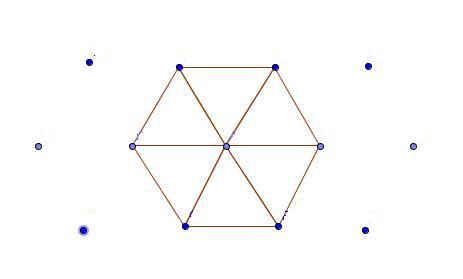
\includegraphics[width=0.5\textwidth]{apunteaklattice}
\caption{$A_{2,\RR^{3}}$}
\end{figure}


\begin{displaymath}
	A_{2,\RR^{3}}=\left\{M'\lambda:\lambda\in\ZZ^{2}\right\}=\left\{\left\begin{bmatrix}
	\lambda_1 \\
	-\lambda_1 + \lambda_2 \\
	-\lambda_2 \end{bmatrix}:\lambda_1,\lambda_2\in\ZZ\right\}
\end{displaymath}

We want to find an hyperplane that contains $A_{2,\RR^{3}}$. We are in $\RR^{3}$, so this hyperplane will be a plane of the form $\left\{x\in\RR^{3}:\left\langle a,x\right\rangle=a_0\right\}$. But we know $0$ is in $A_{2,\RR^{3}}$ so
$H=\left\{x\in\RR^{3}:\left\langle a,x\right\rangle=0\right\}$
$\left\{\omega\in\RR^{3}: \left\langle \omega,x\right\rangle, \forall \in \colospan M\right\}$ where $\colospan M=_\RR\left\langle v_1,\ldots,v_n \right\rangle=im M$ (it is an abelian group and it is also a vector space). So,
$H=\left\{x\in\RR^{3}: \left\langle a,x\right\rangle=0\right\}=\ker M$

$dim \im M=2$ and $dim A_{2,\RR^{3}}=3$ $\Longrightarrow$ $dim A_{2,\RR^{3}}=dim \ker M +dim \im M$ $\Longrightarrow$ $dim \ker M=1$

A generator of $\ker M$ will be $\left(\left[\begin{smallmatrix}
1 \\
1 \\
1 \end{smallmatrix}\right)$

$\left[1 1 1\right]\left[\left[\begin{smallmatrix}
1 & 0 \\
-1 & 1 \\
0 & -1 \end{smallmatrix}\right]=\left[0 0\right]$ $\Rightarrow$ $\ker M= _\RR\left\langle \left[1 1 1\right]\right\rangle$

So $A_{2,\RR^{3}}\subset\left\{x\in\RR^{3}: x_1+x_2+x_3=0\right\}=\left\{x\in\RR^{3}: \mathbbm{1}\right\}$


\begin{definition}
The \emph{Gram matrix} of a lattice $L$ with generator matrix $M$ is $G_L=M^{T}M$.
\end{definition}


\begin{definition}
The \emph{determinant of a lattice} $L$ with generator matrix $M$ is the determinant of the Gram matrix.
$\det L=\det M^{T}\cdot \det M=\left(\det M\right)^{2} $
\end{definition}


\begin{observation}
 $G_L$ is always a symmetric matrix because $G_L^{T}=\left(M^{T}M\right)^{T}=M^{T}M$
\end{observation}


We will see which is the determinant of $A_{2,\RR^{2}}$ and $A_{2,\RR^{3}}$:

$\det A_{2,\RR^{2}}=det \left[\begin{smallmatrix}
1 & 0 \\
1/2 & \sqrt{3}/2 \end{smallmatrix}\right]\cdot\left[\begin{smallmatrix}
1 & 1/2 \\
0 & \sqrt{3}/2 \end{smallmatrix}\right]=\det \left[\begin{smallmatrix}
1 & 1/2 \\
1/2 & 1 \end{smallmatrix}\right]=3/4$

$\det A_{2,\RR^{3}}=\det \left[\begin{smallmatrix}
0 & -1 & 0 \\
0 & 1 & -1\end{smallmatrix}\right]\cdot\left[\begin{smallmatrix}
1 & 0 \\
-1 & 1 \\
0 & -1 \end{smallmatrix}\right]=\det \left[\begin{smallmatrix}
2 & -1 \\
-1 & 2 \end{smallmatrix}\right]=3$


\begin{definition}
The \emph{minimum norm} of a lattice $L$ is $\mu_L=\min\left\{\left\|v\right\|^{2}:v\in L\backslash \left\{0\right\}\right\}$
\end{definition}


The minimum norms of $A_{2,\RR^{2}}$ and $A_{2,\RR^{3}}$ are

$\mu_{A_{2,\RR^{2}}} = 1$

$\mu_{A_{2,\RR^{3}}} = 1$

The determinants and the minimum norms of $A_{2,\RR^{2}}$ and $A_{2,\RR^{3}}$ are different.


\begin{definition}
Two lattices are \emph{isomorphic} if one is obtained from the other by rotation, reflection, translation and sceling.
\end{definition}


We look now to the packing density of $A_{2,\RR^{2}}$ and $A_{2,\RR^{3}}$:

Packing density of L: 

$\Delta_L=\frac{\vol(sphere in packing)}{\vol(\Pi_L)=\sqrt{detL}}$

where $\Pi_L=\left\{\sum\lambda_i v_i : \lambda_i\in\left[0,1\right)\right\}$ is the fundamental parallelpeptide.


In $A_{2,\RR^{2}}$ the radius of the sphere is $\frac{1}{2}$ so the volume is $\left(\frac{1}{2}\right)^{2}\pi$.

$\Delta_{A_{2,\RR^{2}}}=\frac{\left(\frac{1}{2}\right)^{2}\pi}{\sqrt{\frac{3}{4}}}=\frac{\pi}{2\sqrt{3}}$

$\Delta_{A_{2,\RR^{3}}}=\frac{\left(\frac{1}{2}\sqrt{2}\right)^{2}\pi}{\sqrt{3}}=\frac{\pi}{2\sqrt{3}}$

So the lattices are the same.

The most general map between equivalent lattices is $x\longmapsto\alpha A+t$, $t\in\RR^{n}$, $A\in O(n)$, $\alpha\in\RR^{*}$ (the negative are the reflections).

In our case,

$\left[\begin{smallmatrix}
1 & \frac{-1}{\sqrt{3}} \\
-1 & \sqrt{3} \\
0 & \frac{-2}{\sqrt{3}}\end{smallmatrix}\right]\left[\begin{smallmatrix}
1 & \frac{1}{2} \\
0 & \frac{\sqrt{3}}{2}\end{smallmatrix}\right]=\left[\begin{smallmatrix}
1 & 0 \\
-1 & 1 \\
0 & 1\end{smallmatrix}\right]$

So, we have two different ways to write the same lattice. The advantages of $M'$ over $M$ are that the coordinates are nicer and the symmetries of the lattice are more easily seen.


\begin{claim}
Any permutation of the coordinate axes in $\RR^{3}$ is a symmetry of $A_{2,\RR^{3}}$.
\end{claim}


\begin{proof}
Let $P:\RR^{2}\longmapsto\RR^{3}$ be a symmetry, i.e. $P(L)=L\Rightarrow\forall x\in L, P(x)\in L \Rightarrow\forall\lambda\in\ZZ^{2}, \exists\beta\in\ZZ^{2}:PM\lambda=M\beta$ ($x=M\lambda$).

We want to proof that, if $P$ is a permutation then $\forall\lambda\in\ZZ^{2}$ we can find a $\beta$ where this is true.
We know $P$, $M$ and $\lambda$, so we have to find $\beta$. This is a linear equation for $\beta$.
We must show that the linear equation $M\beta=b$ has a unique solution for any $b_\lambda =PM\lambda$.
The solution is unique if $\rank M$ is maximal, i.e. $\rank M=2$.
$M$ has rank 2 so we only have to see if it always has a solution.
For the fundamental theorem of linear algebra part 2 the system has a solution $\Longleftrightarrow$ $b\in \colspan M=\im M$ $\Longleftrightarrow$ $b\bot\left(\colspan M\right)^{\bot} $ $\Longleftrightarrow$ $b^{T}y=0$ whenever $y\bot \colspan M$ $\Longleftrightarrow$ $b^{T}y=0$ whenever $y^{T}M=0$

Let $\left[0 0\right]=\left[y_1 y_2 y_3\right]\left[\begin{smallmatrix}
1 & 0 \\
-1 & 1 \\
0 & -1\end{smallmatrix}\right]=\left[y_1 - y_2, y_2 - y_3\right]$

$y^{T}M=0$ $\Longleftrightarrow$ $y=\alpha\mathbbm{1}$
$b^{T}y=\lambda^{T}M^{T}P^{T}\alpha\mathbbm{1}=\alpha\lambda^{T}M^{T}P^{T}\mathbbm{1}=\alpha\lambda^{T}M^{T}\mathbbm{1}=0$
$M^{T}\mathbbm{1}=0$ because $\mathbbm{1}$ is in the $\ker$ of $M$.
\end{proof}


\subsection{Laminated lattices}


Define $\mathbb{L}_0=\left\{L^{0}\right\}$, $L^{0}=\left\{0\right\}=\mathbb{R}^{0}$ the zero dimensional lattice and $m:=4$ (usually $m$ is 4 because the sphere has radius 1).

For $n>>0$, $\mathbb{L}_{n+1}=\left\{L_1^{n+1},\ldots,L_{a_n}^{n+1}\right\}$ is the collection of $n+1$-dimensional lattices such that
\begin{enumerate}
\item each $L_i^{n+1}$ has constant minimal norm $m$
\item each $L_i^{n+1}$ contains at least ones $L_j^n$ as a sublattice
\item each $L_i^{n+1}$ has minimal determinant subject to (1), (2)
\end{enumerate}


We will see which are this lattices:

\begin{enumerate}
\item $\mathbb{L}_1$ : $k\ZZ$

It needs minimal norm m=4 $\Rightarrow$ $2\ZZ$ 
It satisfies (2) and (3).
So the unique laminates lattice of rank 1 is $2\ZZ$.


\item $\mathbb{L}_2$ :

$M=\left[\begin{smallmatrix}
2 & 0 \\
0 & 2\end{smallmatrix}\right]$ 

Satisfies (1),(2) and (3). It is $2\ZZ^{2}$.


We don't need to use integer points, it only needs to contain $2\ZZ$.

We have two candidates:  $2\ZZ^{2}$ and $A^{2}$. We will see which of them is what we need:

$\det 2\ZZ^{2}=\det M^{T}M=\det\left[\begin{smallmatrix}
4 & 0 \\
0 & 4 \end{smallmatrix}\right]=16$ where $M=\left[\begin{smallmatrix}
4 & 0 \\
0 & 4 \end{smallmatrix}\right]$.

$\det A^{2}=\detM^{T}M=\det\left[\begin{smallmatrix}
4 & 2 \\
2 & 4 \end{smallmatrix}\right]=12$ where $M=\left[\begin{smallmatrix}
2 & 1 \\
0 & \sqrt{3} \end{smallmatrix}\right]$.


$\det A_2 < \det 2\ZZ^{2}$

The area of the parallelpeptide is less than the square. So $\mathbb{L}_2$ will be $A_2$.
\end{enumerate}
We will see now how can we do the sphere packing:

\begin{figure}[htbp]
\centering
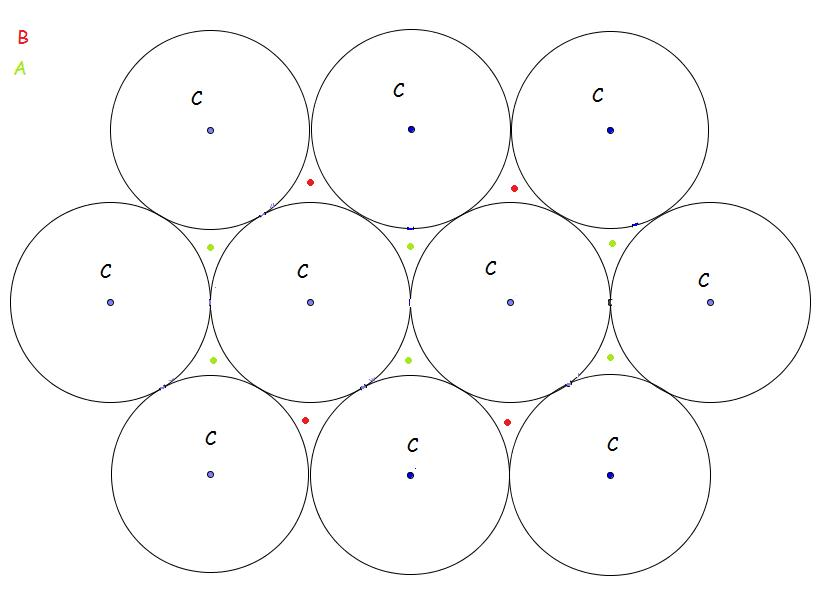
\includegraphics[width=0.5\textwidth]{apunteslattice}
\caption{sphere packing}
\end{figure}

For the next layer we have two options, put them (the centers of the sphere) over the deep holes A or over the deep holes B. For the second layer we put, we will have the possibility of putting them over C (the centers of the spheres of the first layer).
Each lattice obtained by snugly packing copies of $A_2$ is determied by the sequences
ABAB.... (this is the hexagonal close packing(He attoms))
ABCABC....(this is the face-centered cubic lattice ($A_3$))
of equivalence classes of deep holes.

In each step there are two options to choose from, which makes uncountable many possibilities in total.



\chapter{Lattice points in multiples of politopes}

\scribe{Xavier Tapia}

Let's define $L_P(t)= \sharp \{tP^{d} \cap \ZZ ^{d} \}$, this number is equal to $\sharp\{P^{d} \cap \frac{1}{t} \ZZ ^{d}\}$ where $P$ is a polytope.
Take now $P^{o}=int P$ as a topological space, and consider $L_{P^{o}}(t)= \sharp \{t(P^{o})^{d} \cap \ZZ ^{d} \}$.

Let's considerer first some examples of this:

If we take $d=2$ and $t=2$ we will have $9$ points
% DIBUJO DE 2 CUADRADO%

Considerer some tables.

\begin{table}[ht]
\centering
\begin{tabular}{c|c|c|c|c|c|c|c}
 & 0 & 1 & 2 & 3 & 4 & ... & t \\
 \hline
$L_{\Box^2}(t)$ & 1 & 4 & 9 & 16 & 25 & ... & $(t+1)^{2}$\\
\hline
$L_{(\Box^2)^0}(t)$  & 0 & 0 & 1 & 4 & 9 & ... & $(t-1)^{2}$\\
\hline
$L_{\Box^1}(t)$ & 1 & 2 & 3 & 4 & 5 & ... & $t+1$ \\
\hline
$L_{(\Box^1)^0}(t)$ & 0 & 0 & 1 & 2 & 3 & ... & $t-1$ \\
\end{tabular}
\end{table}

It's possible to see that, in general:

\begin{theorem}
$L_{\Box^d}(t) = (t+1)^{d}$, $L_{(\Box^d)^0}(t)=(t-1)^{d}=(-1)^{d}L_{\Box^d}(-t)$
\end{theorem}

In fact, this result is true for every polytope $P$ not only for $\Box^d$, this theorem is known as the Ehrart-Macdonald Reciprocity and it's the principal result we want to prove.

\begin{theorem}[Ehrhart-Macdonald Reciprocity]
\[
  L_P(-t) = (-1)^d L_{P^0}(t)
\]
\end{theorem}

To proof this theorem we need some previous results,

\section{Generating functions for rational cones}

Take $S$ a rational cone or polytope (i.e. the generators of $1$-$d$ rays with rational vertices coordinates). We define:

$$G_S(z)=G_S(z_1,z_2,...,z_d)= \sum _{m \in S \cap \ZZ ^{d}} z^{m}=\sum _{m \in S \cap \ZZ ^{d}} z_1^{m_1}...z_d^{m_d}$$

$G(z)=1+x+y+xy=(1+x)(1+y)$

Goal: Find $G_c(z)$ where $ C=\{v_1,...,v_d\} \subset \\R ^{d}$

Assume that $C$ is simplicial (that0s mean $C$ is a cone over a simplex), so the paralelopiped $\Pi_C=\{\lambda_1v_1+...+\lambda_dv_d : 0 \leq \lambda_i \leq 1\}$ till $C$ disjointlly.

In particullar, $G_C(z)= \sum_{s_i \in \NN} tr_{\sum s_iv_i}G_{\Pi}(z)=\sum_{s_i \in \NN} z^{\sum s_iv_i}G_{\Pi}(z)=\frac{G_{\Pi}(z)}{(1-z^{v_1})...(1-z^{v_d})} \in \QQ[[z_1,...,z_d]]$ 

\begin{theorem}[Beck-Robins theorem 3.5]
Suppose $C=cone\{v_1,...,v_d\}$ cone over a simplex, then for all $v \in \RR^{d}$ the generating function satisfies:

$$G_{v+C}=\frac{G_{v+\Pi_C(z)}}{(1-z^{v_1})...(1-z^{v_d})}$$
\end{theorem}

\begin{proof}
In $G_{v+C}(z)=\sum_{m \in (v+C) \cap \ZZ ^{d}} z^{m}$ write $m=w+\lambda_1v_1+...+\lambda_dv_d$ for $\lambda_i \geq 0$, and take $\lambda_k= \lfloor \lambda_k \rfloor+\lbrace \lambda_k \rbrace$ so for that, we can write:
$$m=w+\lfloor \lambda_1 \rfloor v_1+...+\lfloor \lambda_d \rfloor v_d+\lbrace\lambda_1 \rbrace v_1+...+\lbrace\lambda_d \rbrace v_d$$

The vector $P=w+\lbrace\lambda_1 \rbrace v_1+...+\lbrace\lambda_d \rbrace v_d \in \ZZ^{d}$ is unique and any $u \in v+C\cap \ZZ^{d}$ can be written uniquely as $P+\sum n_i v_i$ with $P\in \Pi_C$ and $n_i \in \ZZ$.

We have:

$$\frac{\sigma_{w+\Pi_C}(z)}{(1-z^{v_1})...(1-z^{v_d})}=\left(\sum_{m \in (v+C) \cap \ZZ ^{d}+w} z^{m}\right)\left(\sum_{k_i \in \NN} z^{k_1 v_1}\right)...\left(\sum_{k_d \in \NN} z^{k_d v_d}\right)$$

Note that if $\Delta C \cap \ZZ^{d}=\phi$ it suffices to take $\Pi_C^{0}=\{\sum_{i=1}^{d} \lambda_i v_i, 0<\lambda_i<1\}$ the open fundamental paralelopiped.
\end{proof}

\begin{theorem}
For any pointed cone (it's maximum linear subspace contained in $C$ is $\{ 0 \}$) $C=\{w+\sum \lambda_i v_i, \lambda_i \geq 0 \}$ with $w \in \RR^{d}$ and $v_i \in \ZZ^{d}$, the generating function $\sigma_C (z)$ is a rational function in the $z_i$.
\end{theorem}
\setcounter{chapter}{7}
\chapter{Introduction to orbifolds}
\scribe{Ane Santos}

\begin{definition}
Informally, an \emph{orbifold} is the quotient of a manifold (here, the Euclidean plane) by the action of a group.
\end{definition}

\begin{center}
	\begin{tabular}{lcc}
		torus & $\longleftrightarrow$ & \bc \\
		holes & $\longleftrightarrow$ & \rs \\
		non-orientability & $\longleftrightarrow$ & \rt \\
		boundary singularity & $\longleftrightarrow$ & \rs\rn \\
		cone point of order $n$ & $\longleftrightarrow$ & \bn \
	\end{tabular}
\end{center}

\begin{theorem}[Magic theorem for the sphere]
The total cost of the signature of any spherical group is $ \$ 2-\frac{2}{g}$, where
$g$~denotes the total number of symmetries.
\end{theorem}

The Magic theorem in the plane is a special case because the number of symmetries in a plane is infinite, so the cost is always 2.

There are 14 spherical symmetry groups: $m,n\geq1$

\begin{center}
	\begin{tabular}{lcccc}
		\crb{*532} & \crb{*432} & \crb{*332} & \crb{*22n} & \crb{*mn} \\
		 & & \cbb{3}\crb{*2} & \cbb{2}\crb{*n} & \cbb{n}\crb{*} \\
		 & & & & \cbb{n}\rt \\
		 \cbb{532} & \cbb{432} & \cbb{332} & \cbb{22n} & \cbb{mn} 
	\end{tabular}
\end{center}

If $n\rightarrow\infty$ and $m\rightarrow\infty$ in \crb{*22n}, \crb{*mn}, \cbb{2}\crb{*n}, \cbb{n}\rs, \bn\rt, \cbb{22n} and \cbb{mn} we get the 7 possible groups of friezes (cenefas).

\bigskip
We spent almost the entire lecture with scissors and tape, cutting out the orbifolds corresponding to the
tesselations in~\cite{Conway-Strauss08}.


% Local Variables: 
% mode: latex
% TeX-master: "dag-upc"
% End: 

\chapter{Orbifolds}

\scribe{Roger Ten}

\section{Defining an orbifold}

In this section $X$ denotes a topological space and $G$ denotes a topological group. So must begin by defining what is a topological group.\\

\begin{defn}

\begin{enumerate}
\item A \underline{topological group} is a topological space that is simultaneously a group such that, the group operations are continuous.
\item A topological space $X$ is called \underline{$G$-space} if a topological group $G$ acts on $X$ via a continuous map $\begin{array}[c]{ccc}
 G\times X&\rightarrow &X\\
(g,x)&{\rightarrow}& gx
\end{array}$ such that
\begin{enumerate}
  \item  $g(hx)=(gh)x$
  \item $1_Gx=x$
\end{enumerate}
\end{enumerate}
\end{defn}

\begin{example}

\begin{itemize}
  \item Lie groups: $O(n), SO(n)$
  \item $S^1$ is a topological space and it is also a group via:
  $$\begin{array}[c]{cccc}
 +: &S^1\times S^1&{\rightarrow}&S^1\\
&(\varphi,\Psi)&{\rightarrow}& \varphi +\Psi
\end{array}$$
\begin{center}
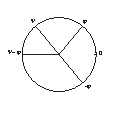
\includegraphics[width=0.5\textwidth]{./suma}
\end{center}
\end{itemize}

\end{example}

Now is coming a list of definitions
\begin{defn}
Let be $x\in X$.
\begin{enumerate}
\item $G_x=\{g\in G : gx=x\}=Stab_G(x)$ is called the \underline{stabilizer of $x$} or the isotropy subgroup of $x$. $G_x$ is a subgroup of $G$ $(G_x\leqslant G).$
\item $G(x)=\{gx : g\in G\}\subset X$ is the \underline{orbit of $x$}.
\item The action of $G$ on $X$ is \underline{free} if $G_x=\{ 1\} \forall x\in X.$
\item The action of $G$ on $X$ is \underline{transitive} if $G(x)=X \forall x\in X$, i.e., there exist only one orbit.
\item The map $G/G_x\rightarrow G(x)$ is a continuous bijection
\item The orbit space $X/G$ is the set of all orbits in $X$. (It is a topological space with quocient topology).
\item A map $f:X\rightarrow Y$ of $G$-spaces is \underline{$G$-equivariant} (or $G$-map) if $f(gx)=g(f(x)); g\in G$. so the following diagram commutes:
 $$\begin{array}[c]{ccc}
X&\stackrel{f}{\rightarrow}&Y\\
\downarrow\scriptstyle{g}&\circlearrowright&\downarrow\scriptstyle{g}\\
X&\stackrel{f}{\rightarrow}&Y
\end{array}$$
\end{enumerate}
\end{defn}

%---------------------------------------------------- Orbifold Chart

\begin{defn}
An \underline{orbifold chart} on a topological space $X$ is tuple $(\tU,G,\cU, \pi)$, such that:
\begin{itemize}
  \item $\cU\subset X$ is an open subset (neighborhood).
  \item $\tU\subset \RR^n$ is an open subset.
  \item $G$ is a finite group of homomorphisms of  $\tU$.
  \item $\pi:\tU\rightarrow \cU$ can be factorized as $\pi=\tilde{\pi}\circ p$, where 
  $p:\tU\rightarrow \tU/G$ is the orbit map and $\tilde{\pi}:\tU/G\rightarrow \tU$ is an homomorphism.
\end{itemize}
\end{defn}





\begin{tikzpicture}[>=angle 90]
\matrix[matrix of math nodes,row sep=3em, column sep=0.25em,
text height=1.5ex, text depth=0.25ex]
{G&\underset{act\ on}{\circlearrowleft} &|[name=tU]| \tU &\subset &\RR^n \\
     &    &           & &|[name=tUG]| \tU/G \\
& & |[name=U]| \cU & \subset &X \\};
\draw [->,font=\scriptsize]
(tU) edge node[auto] {$p$} (tUG)
(tU) edge node[auto] {$\pi$} (U)
(tUG) edge node[auto] {$\tilde{\pi}$} (U);
\end{tikzpicture}

 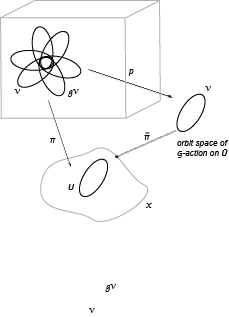
\includegraphics[width=0.5\textwidth]{./orbitchart}



\begin{defn} Two orbifold charts are \underline{compatible} if $\forall \tilde{u_i}\in \tU_i, i=1,2$ $\pi_1(\tilde{u_1})=\pi_2(\tilde{u_2})$  then exist an homomorphism $h:\tV_1\rightarrow\tV_2$ where $\tV_i$ is a neighborhood of $\tilde{u_i}$ in $\tU_i$, such that $\pi_1=\pi_2\circ h$ on $\tV_1$

\begin{center}
\begin{tikzpicture}[>=angle 90]
\matrix[matrix of math nodes,row sep=1em, column sep=0.5em,
text height=1.5ex, text depth=0.25ex]
{|[name=U2]|\tU_2&\supset &|[name=V2]| \tV_2 & &|[name=V1]|\tV_1&\subset &|[name=U1]| \tU_1 \\
&&&\circlearrowright &&&\\
|[name=U2G]|\tU_2/G& & &|[name=U1U2]| \tU_1\cap\tU_2 & & &|[name=U1G]| \tU_1/G0\\};
\draw [->,font=\scriptsize]
(V1) edge node[auto] {$h$} (V2)
(V1) edge node[auto] {$\pi_1$} (U1U2)
(V2) edge node[auto] {$\pi_2$} (U1U2)
(U1G) edge node[auto] {$\tilde{\pi}_1$} (U1U2)
(U2G) edge node[auto] {$\tilde{\pi}_2$} (U1U2)
(U1) edge node[auto] {$p_1$} (U1G)
(U2) edge node[auto] {$p_2$} (U2G);
\end{tikzpicture}
\end{center}
\end{defn}

\begin{remark}
$G_i=\{1\}$ yields manifolds
\end{remark}

\begin{defn}
An \underline{orbifold atlas} is a collection of compatibles orbifold charts that cover $X$.\\
An \underline{orbifold $Q$} is an underlying Haursdorff topological space $|Q|$ with an orbifold atlas.
\end{defn}

\section{Covering orbifolds}

A covering of a topological space $X$ is a topological space $Y$, together with a continuous surjective projection $\pi: Y\rightarrow X$ such that for every $x\in X$ exist $\cU_x$ open neighborhood of $x$ such that the pre-image $\pi^{-1}(\cU_x)$ is a disjoint union of copies of $\cU_x$.


\begin{defn}
A \underline{covering orbifold} of an orbifold $Q$ is an orbifold $\tilde{Q}$ with a projection $\pi:|\tilde{Q}|\rightarrow|Q|$ between the underlying spaces with the following property:
\begin{description}
  \item[] For any $x\in |Q|$ there exist a neighborhood $\cU\cong \tU/G$; $\cU\subset \RR^n$ such that each connected component $C$ of $\pi^{-1}(\cU)$ is homeomorphism to $\tU/\Gamma_i$ for some subgroup $\Gamma_i\leqslant G$.
\end{description}
\end{defn}
\begin{remark}
This homeomorphism $\varphi$ must respect both projections, namely $\pi$ and $p_i:\tU/G\rightarrow\tU/\Gamma_i$.

\begin{tikzpicture}[>=angle 90]
\matrix[matrix of math nodes,row sep=1em, column sep=3em,
text height=1.5ex, text depth=0.25ex]
{&&&&\\
|[name=tQ]| |\tilde{Q}|&|[name=C]| 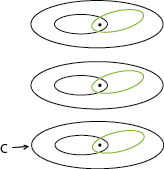
\includegraphics[width=0.15\textwidth]{./C} & &|[name=tU]|\tU &|[name=tUd]| 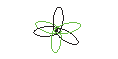
\includegraphics[width=0.15\textwidth]{./tU} \\
&&&&\\
 &&\circlearrowright & |[name=tUG]| \tU/G& |[name=tUGd]| \\
|[name=Q]| |Q|&|[name=U]|  \cU & & &
\includegraphics[width=0.15\textwidth]{./tUG} \\
&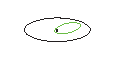
\includegraphics[width=0.15\textwidth]{./U}&&&\\};
\draw [->,font=\scriptsize]
(tQ) edge node[auto] {$\pi$} (Q)
(C) edge node[auto] {$\pi$} (U)
(tUG) edge node[auto] {$\tilde{\pi}$} (U)
(tU) edge node[auto] {$\varphi$} (C)
(tU) edge node[auto] {$p$} (tUG)
(tUd) edge node[auto] {$p$} (tUGd);
\end{tikzpicture}


\end{remark}

\begin{defn}
An orbifold is called \underline{good} or developable if there exists some manifold that covers it. Otherwise, it is \underline{bad} or not developable
\end{defn}








\chapter{The Magic Theorem}

\scribe{Victor Bravo}

Today, we want to prove the Magic Theorem. To do this, we will introduce the language of the CW-Complexes: \newline

\underline{CW-COMPLEXES:}
\begin{obs} The theory of CW-Complexes was developed around 1910 by J.H.\underline{C}. \underline{W}hitehead. Also, the 'C' do refence to 'closed' and the 'W' do reference to 'weak' in the sentence 'closed in the weak topology'. \newline
We will use CW-Complexes to generalize triangulations of the space.
\end{obs}

Let $X$ be a topological space. \newline
We define $X^{0} := 0$-skeleton of $X = \lbrace \text{points in } X \rbrace$. \newline
Inductively, given the $(n-1)$-skeleton of $X$, take a bunch of $n$-dimensional closed disks ($\equiv$ balls) $e_{1}^{n}, \ldots, e_{r}^{n}$, and we can do the next attaching map $\varphi _{i} : \mathbb{S}^{n - 1} = \partial e_{i}^{n} \longrightarrow X^{n - 1}$. \newline
$X^{n} := X^{n-1} \stackrel{\bullet}{\bigcup}_{i} e_{i}^{n} / \sim$, where $x \sim \varphi_{i}(x)$. \newline
Since a $1$-dimensional disk is an interval, taking a set of points in a plane, a $1$-dimensional CW-Complex is a multigraph with loops. \newline
In dimension $2$, a good example can be to take only the point $p$ as the $0$-skeleton, an empty number of $1$-dimensional balls, and a $2$-dimensional ball (which is a disk). So, we have that the attaching map goes from the boundary of this disk (which is $\partial e^{2} = \mathbb{S}^{1}$) to the lower dimensional skeleton (which is the point $p$). Doing the $\sim$, we get the $2$-dimensional sphere. \newline
The same example works for any dimension $n$ using stereographic projection. So, we can calculate the number of cells that we need to decomposing $\mathbb{S}^{n}$ as a regular triangulation (regular in the sense of not having identifications on the boundary of the cell and in the sense of the intersection of two faces is empty or a face of both). \newline
For dimension $0$, we have two points. So, the $f$-vector of $\mathbb{S}^{0}$ is $(2)$ (which means: two $0$-dimensional faces), and we need $(2)$ cells in the CW-complex. \newline
For dimension $1$, we have $\mathbb{S}^{1}$ and, to do a regular triangulation, we need three different distinguished points. So, the $f$-vector of $\mathbb{S}^{1}$ is $(3, 3)$ (which means: three $0$-dimensional faces and three $1$-dimensional faces), and we need $(1, 1)$ cells in the CW-complex. \newline
For dimension $2$, we have $\mathbb{S}^{2}$ and, to do a regular triangulation, we need a tetrahedron over the $\mathbb{S}^{2}$ surface. So, the $f$-vector of $\mathbb{S}^{2}$ is formed by $4$ vertices, $\binom{4}{2}$ edges, and $\binom{4}{3}$ faces (triangles). This is $(4, 6, 4)$, and we need $(1, 0, 1)$ cells in the CW-complex. \newline
For dimension $n$, we have the $n$-dimensional simplex. So, whose $f$-vector is equal to $(n + 1, \binom{n+1}{2}, \binom{n+1}{3}, \ldots, \binom{n+1}{n})$ (that has $2^{n+1}-2$ elements), and we need $(1, 0, \ldots, 0, 1)$ cells in the CW-complex. \newline

To go towards the Magic Theorem, we need to remember the definition of the covering of an orbifold to explain: \newline

\underline{THE ORBIFOLD EULER CHARACTERISTIC:} \newline \newline
Let be $G$ a group that acts over an orbifold $Q$, $G \circlearrowleft Q$. \newline
So, taking $x \in Q$, we have that $G_{x} \leq G$ is that we call the stabilizer of $x$. \newline
What we want to do is to decompose $Q$ as a CW-complex into invariant cells, i.e., into a collection, $\mathcal{C}$, of cells such that the function $x \mapsto G_{x}$ is constant on each cell, $C \in \mathcal{C}$ (observe that $C^{0} \subset C$). \newline
An example of this is to take $\vert Q \vert = \mathbb{D}^{2}$ and $G$ as the abstract group $G = \lbrace e = id, g, g^{2} \rbrace = \mathbb{Z}_{3}$, where $g$ represents a rotation of $\frac{2 \pi}{3}$ (this is the same that to think in $G$ as the spherical group formed by two rotation points of order three). Now, we want to decompose this as a CW-manifold into cells such that the stabilizing subgroup is constant. We have two differents types of points that we resume as points $y$, which are rotation points, and points $x$ which are not rotation points. Now, the stabilizing group of the points $x$ is $G_{x} = \lbrace e \rbrace$, and the stabilizing group of the points $y$ is $G_{y} = G$. So now, we will have to decompose this disk as a CW-complex made-up of invariant cells. To do this, we have to leave one of the rotation points in the interior of the disk, the other rotation point over the boundary of the disk, and add two new points over the boundary of the disk. \newline
Now, we define the \textsl{Euler Characteristic of an orbifold} as $$\chi (Q) = \sum_{C \in \mathcal{C}} \frac{(-1) \dim C}{\# G_{C}}.$$
To see that this definition works, we have to check two things. \newline
The first thing is that this defition is an application of the original Euler Characte-ristic that works over orbifolds in the same sense of the original works over simplicial complexes, where the original Euler Characteristic is defined as the alternating sum of the $f$-vector of the simplicial complex.
\begin{example} Taking the simplicial complex formed by the three vertices, the three edges and the face of a triangle (i.e., a $2$-dimensional ball), we have to sum $1(-1)^{2}$ for the face, $3(-1)^{1}$ for the edges, $3(-1)^{0}$ for the vertices and $1(-1)^{-1}$ for the $\emptyset$, which gives us $\chi = 0$. \newline
In the same way, if we take the simplicial complex formed by the three vertices, the three edges of a triangle, this gives us $\chi = -1$. \newline
\end{example}

This works for any regular triangulation, so, if works for orbifolds. \newline
The second thing to check is that this formula works for the group, but in the case of having a simplicial complex there is no group, or in other words, we have only the identity. So, it works for the group. \newline
Now, what we really wants is apply this to coverings, so, remember: \newline
In a $k$-fold, covering $\tilde{Q} \rightarrow Q$ of orbifolds, every point in $\vert Q \vert$ has $k$ pre-images. \newline
\begin{theorem} If $\tilde{Q} \rightarrow Q$ is a $k$-fold covering of orbifolds, then $\chi(\tilde{Q}) = k \chi (Q)$.
\end{theorem}
\begin{proof} Remembering session 9, let $y \in U$ be a non-singular point in an orbifold chart, $U$, which corresponds to a some number of points in $V$. \newline
The number of pre-images of $y$ in each neighborhood of $\tilde{x}_{i}$ is $\dfrac{\vert G_{x} \vert}{\vert G_{\tilde{x}} \vert}$. \newline
So, the total number of preimages of $y$ is $$k = \sum_{\tilde{x} \in \Pi ^{-1}(x)} \frac{\vert G_{x} \vert}{\vert G_{\tilde{x}} \vert},$$ which implies that $$\frac{k}{\vert G_{x} \vert} = \sum _{\tilde{x} \in \Pi ^{-1}(x)} \frac{1}{\vert G_{\tilde{x}} \vert}.$$ Now, using that the cells are invariant and $x \mapsto G_{x}$, we have that $$\frac{k}{G_{x}} = \frac{k}{G_{C}}.$$ So, we have that $$k \chi (Q) = \sum_{C \in \mathcal{C}} \frac{k (-1)^{\dim (C)}}{\vert G_{C} \vert} = \sum _{\tilde{C} \in Pi^{-1}(C)} \frac{(-1)^{\dim (C)}}{\vert G_{\tilde{C}} \vert} = \chi (\tilde{Q}),$$ where the last equality holds because $\tilde{C} \in Pi^{-1}(C), \forall C \in \mathcal{C}$, and this sums over all $\tilde{C} \in \vert \tilde{Q} \vert$.
\end{proof}
\qed

\begin{example} Let's take $\vert Q \vert = \mathbb{D}^{2}$ with $k$ mirrors and $k$ corner reflectors  labeled $m_{1}, \ldots, m_{k}$. \newline
If we compute de signature of this, we have no blue part because there are not rotation points. Then, we have a \textcolor{red}{$*$}, and we can take, for example, the signature \textcolor{red}{$*632$}. So, we have one point, $A$, with $6$ mirrors through it, another point, $C$, with $3$ mirrors through it, and another point, $B$, with $2$ mirrors through it. Now, if we go down to the orbifold (taking one copy of every mirror), we have $3$ mirrors in the orbifold. So, $k = 3$. Now, we want to cellulate this CW-complex such that every cell in the CW-complex has the same stabilizer. Since, $A$ is stabilized by the subgroup $D_{6}$, $B$ is stabilized by the subgroup $D_{2}$, and $C$ is stabilized by the subgroup $D_{3}$, we can compute the Orbifold Euler Characteristic. \newline
We have, for dimension $0$, $$\frac{(-1)^{0}}{\vert D_{6} \vert} + \frac{(-1)^{0}}{\vert D_{2} \vert} + \frac{(-1)^{0}}{\vert D_{3} \vert},$$ for dimension $1$, $$\frac{(-1)^{1}}{\vert \mathbb{Z}_{2} \vert} + \frac{(-1)^{1}}{\vert \mathbb{Z}_{2} \vert} + \frac{(-1)^{1}}{\vert \mathbb{Z}_{2} \vert},$$ and for dimension $2$, $$\frac{(-1)^{2}}{\vert \lbrace e \rbrace \vert}.$$ \newline
So, $$\tilde{\chi} = \frac{1}{12} + \frac{1}{4} + \frac{1}{6} - \frac{1}{2} - \frac{1}{2} - \frac{1}{2} + \frac{1}{1} = 0.$$
\end{example}

\begin{example} Doing the same example with any $k$ corner reflectors using the notation $m_{i}$ to note the number of mirrors through the corner $i$, we will have $$\tilde{\chi} = \sum_{i = 1}^{k} \frac{1}{2 m_{i}} - \frac{k}{2} + 1 = \frac{1}{2} \sum_{i = 1}^{k} \left(\frac{1}{m_{i}}\right) + 1 = 1 - \sum_{i=1}^{k} \frac{m_{i} - 1}{2 m_{i}}.$$ So, if we get a disk, it has this Euler Characteristic.
\end{example}

\begin{example} Now, an example with true-blue signature (which means that we have only rotation points). Let's take $\vert Q \vert = \mathbb{S}^{2}$, and $l$ cone points labeled $n_{1}, \ldots, n_{l}$. Let's take, for example, \textcolor{blue}{$532$} over $\mathbb{S}^{2}$. So, we have a sphere and three cone points. The first thing we've got to do is to cellulate the sphere as a CW-complex such that each cell has constant stabilizer. So, it seems very clear that we are going to use $0$-dimensional vertices at the cone points. So, the stabilizing subgroup is $C_{5}$ for one point, $C_{3}$ for another point, and $C_{2}$ for another point. In the same way, the stabilizing subgroup of the edges that goes from one point to another is $\lbrace e \rbrace$, and also for the face, the subgroup is $\lbrace e \rbrace$. So, we have that $$\tilde{\chi} = \frac{(-1)^{0}}{5} + \frac{(-1)^{0}}{3} + \frac{(-1)^{0}}{2} - 1 - 1 - 1 + 1 + 1 = \sum_{i = 1}^{l} \frac{1}{n_{i}} - l + 2 = 2 - \sum_{i = 1}^{l} \frac{n_{i} - 1}{n_{i}}.$$
What we have to observe here is that seems that we extract something from $2$. In the last example seems that happens the same thing, but there we had a \textcolor{red}{$*$} and all was natural. What happens here is that using $\chi({\mathbb{S}^{2}}) = (-1)^{0} + (-1)^{2} = 2$, we have that if we do a hole over the sphere, we are substracting $1$, because $\chi(\mathbb{S}^{2} \text{ with a hole}) = 1$, and we have the possible \textcolor{red}{$*$}'s covered. So, finally we have that $\tilde{\chi}(Q) = 2 - (\text{cost of the signature})$.
\end{example}



% Local Variables: 
% mode: latex
% TeX-master: "dag-upc"
% End: 

\chapter{Quasicrystals}
\begin{figure}[h] %[h] para here [b] para bottom [t] para top
\centering
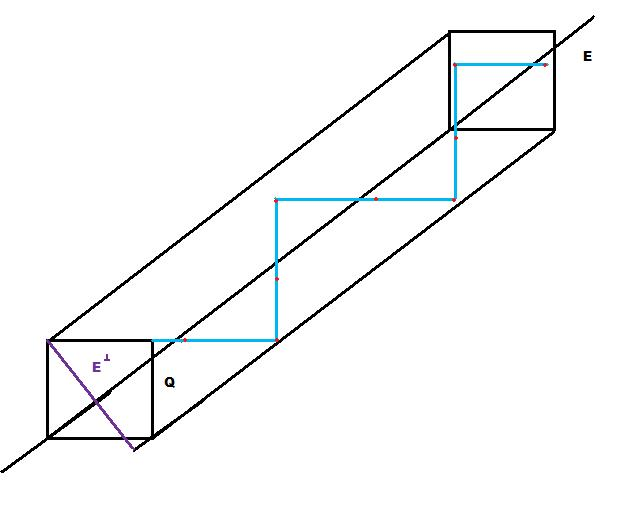
\includegraphics[width=250pt]{./graphics/Quasi.jpg}
%\caption{Ejemplos de cada tipo de juego}
\end{figure}
We pick
$$\textbf{E}=\{\vec{x}\in\RR^2\ |\ x_2=x_1\cdot c,\ c\in\RR\setminus\QQ\}.$$
There are $2$ kind of segments the big ones and the smaller ones the proportion is $c$.\smallskip\\
$\textbf{E}^{\bot}$ is dense $\Rightarrow 2^{\NN}$ is $\infty$ no countable.\smallskip\\
We can generalize this to any parallelepiped and if we are in a lattice the canonical projetion method picks $\Vor(0)$ as $Q$. It is also possible in higher dimensions.\smallskip\\
Given $x\in L$, $\textbf{E}\subset \RR^d$, $Q\subseteq\RR^d$ we have to decide whether $x\in\mathbf{E}+Q$.\smallskip\\
We project $Q$ and $x$ onto $\pi_{\textbf{E}^{\bot}}(\mathbf{E}+Q)$, where $\pi_{\textbf{E}^{\bot}}$ is the projection window, if $x^{'}\in Q^{'}\Leftrightarrow x\in\mathbf{E}+Q$.

\bibliographystyle{amsalpha}
\bibliography{dag}

\end{document}

%%% Local Variables: 
%%% mode: latex
%%% TeX-master: t
%%% End: 
